\chapter{人类生殖}\label{ch:g5:human-reproduction}

你认识的每一个人——朋友、老师、你家中最年长的人——
都是以同样的方式来到世上的：作为婴儿，
在母亲体内生长数月后降生。人类是\omterm{prop:g3:sorting-living-things:groups}{哺乳动物}
（\cref{prop:g4:classifying-animals:classes}），人类生殖
沿用\cref{ch:g4:animal-reproduction}中的\omterm{prop:g3:sorting-living-things:groups}{哺乳动物}模式，
但带有人类这一\omterm{def:g5:biodiversity:species}{物种}的具体数字、日期
和各种细节，
本章将清楚地予以介绍。

\section{人类生殖的模式}

\begin{proposition}[人类生殖就是哺乳动物的生殖]\label{prop:g5:human-reproduction:plan}
与所有\omterm{prop:g3:sorting-living-things:groups}{哺乳动物}一样，人类进行\omterm{def:g4:animal-reproduction:sexual}{有性生殖}
（\cref{def:g4:animal-reproduction:sexual}）：
\begin{itemize}
  \item 母体产生\emph{\omterm{def:g4:animal-reproduction:sexual}{卵细胞}}；
        父体产生\emph{\omterm{def:g4:animal-reproduction:sexual}{精子}}；
  \item \omterm{def:g5:flower-to-fruit:steps}{受精}——一个\omterm{def:g4:animal-reproduction:sexual}{精子}与一个\omterm{def:g4:animal-reproduction:sexual}{卵细胞}结合
        ——发生在\emph{母体内}
        （\cref{prop:g4:animal-reproduction:where}）；
  \item \omterm{def:g5:flower-to-fruit:steps}{受精}卵——一个单\omterm{def:g5:first-look-at-cells:cell}{细胞}
        （\cref{ex:g5:first-look-at-cells:one}）——附着于
        母体的\emph{子宫}\index{子宫}中并在那里生长；
  \item 人类是\omterm{def:g4:animal-reproduction:ovivivi}{胎生}的
        （\cref{def:g4:animal-reproduction:ovivivi}）：婴儿
        \omterm{def:g2:animals-grow-up:born}{胎生出生}，最初以\omterm{def:g2:animals-grow-up:born}{乳汁}喂养。
\end{itemize}
\end{proposition}
\admitted

\begin{remark}[生殖需要成年人的身体]\label{rem:g5:human-reproduction:adults}
儿童的身体还不能生育：生殖器官
要到\emph{青春期}才开始工作。青春期是
\cref{def:g3:stages-of-life:stages}中青少年阶段的转变，
身体由儿童转变为成人。青春期会发生
哪些变化、如何变化，
将在本书的初中阶段专章详述。
\end{remark}

\section{子宫中的九个月}

\begin{definition}[怀孕]\label{def:g5:human-reproduction:pregnancy}
\emph{怀孕}\index{怀孕}是未来婴儿在母亲\omterm{prop:g5:human-reproduction:plan}{子宫}中
生长的时期，人类约为\emph{九个月}。
生长中的婴儿最初称为
\emph{胚胎}\index{胚胎}，
待身体结构基本形成（约两个月后），
便称为\emph{胎儿}\index{胎儿}。
\end{definition}

\begin{proposition}[通过脐带获得营养]\label{prop:g5:human-reproduction:cord}
在\omterm{prop:g5:human-reproduction:plan}{子宫}内，婴儿漂浮在一小袋液体中，
既不能进食，也不能\omterm{def:g4:breathing:movements}{呼吸}。一切所需都
来自母亲的\omterm{prop:g4:journey-of-food:absorb}{血液}：\omterm{def:g4:journey-of-food:digestion}{营养物质}和氧气
（\cref{prop:g4:heart-and-blood:carries}）经
由婴儿腹部的
\emph{脐带}\index{脐带}进入婴儿\omterm{prop:g4:journey-of-food:absorb}{血液}，
废物则以同样方式返回，由母体处理。
你的肚脐就是你自己\omterm{prop:g5:human-reproduction:cord}{脐带}的附着之处。
\end{proposition}
\admitted

\begin{example}[九个月的时间表]\label{ex:g5:human-reproduction:timetable}
第 1 个月：一团正在分裂的\omterm{def:g5:first-look-at-cells:cell}{细胞}，比一粒米还小，
但已快速生长。第 2 个月：\omterm{def:g5:human-reproduction:pregnancy}{胚胎}已有
头部雏形、跳动的\omterm{def:g4:heart-and-blood:heart}{心脏}，以及手臂和腿的芽——
仍比拇指还小。第 3 至 4 个月：\omterm{def:g5:human-reproduction:pregnancy}{胎儿}结构已基本齐全，
开始活动；母亲很快就能感受到胎动。
第 5 至 8 个月：继续生长发育——听觉形成，身上
长出一层细毛。第 9 个月：婴儿通常头朝下，
体重约 \qty{3}{kg}，已经准备就绪。
\end{example}

\begin{example}[出生]\label{ex:g5:human-reproduction:birth}
分娩时，\omterm{prop:g5:human-reproduction:plan}{子宫}有力的\omterm{def:g3:bones-and-muscles:muscle}{肌肉}将婴儿推出母体，
通常是头先出来。第一声啼哭将空气充入肺中
——在此之前它们从未\omterm{def:g4:breathing:movements}{呼吸}过
（\cref{prop:g5:human-reproduction:cord}）。\omterm{prop:g5:human-reproduction:cord}{脐带}已不再需要，
被无痛地剪断，\omterm{prop:g3:sorting-living-things:groups}{哺乳动物}的生殖模式在体外延续：
\omterm{def:g2:animals-grow-up:born}{乳汁}、温暖和照顾
（\cref{ex:g4:animal-reproduction:whalecalf}对此也会认同）。
\end{example}

\begin{omfigure}
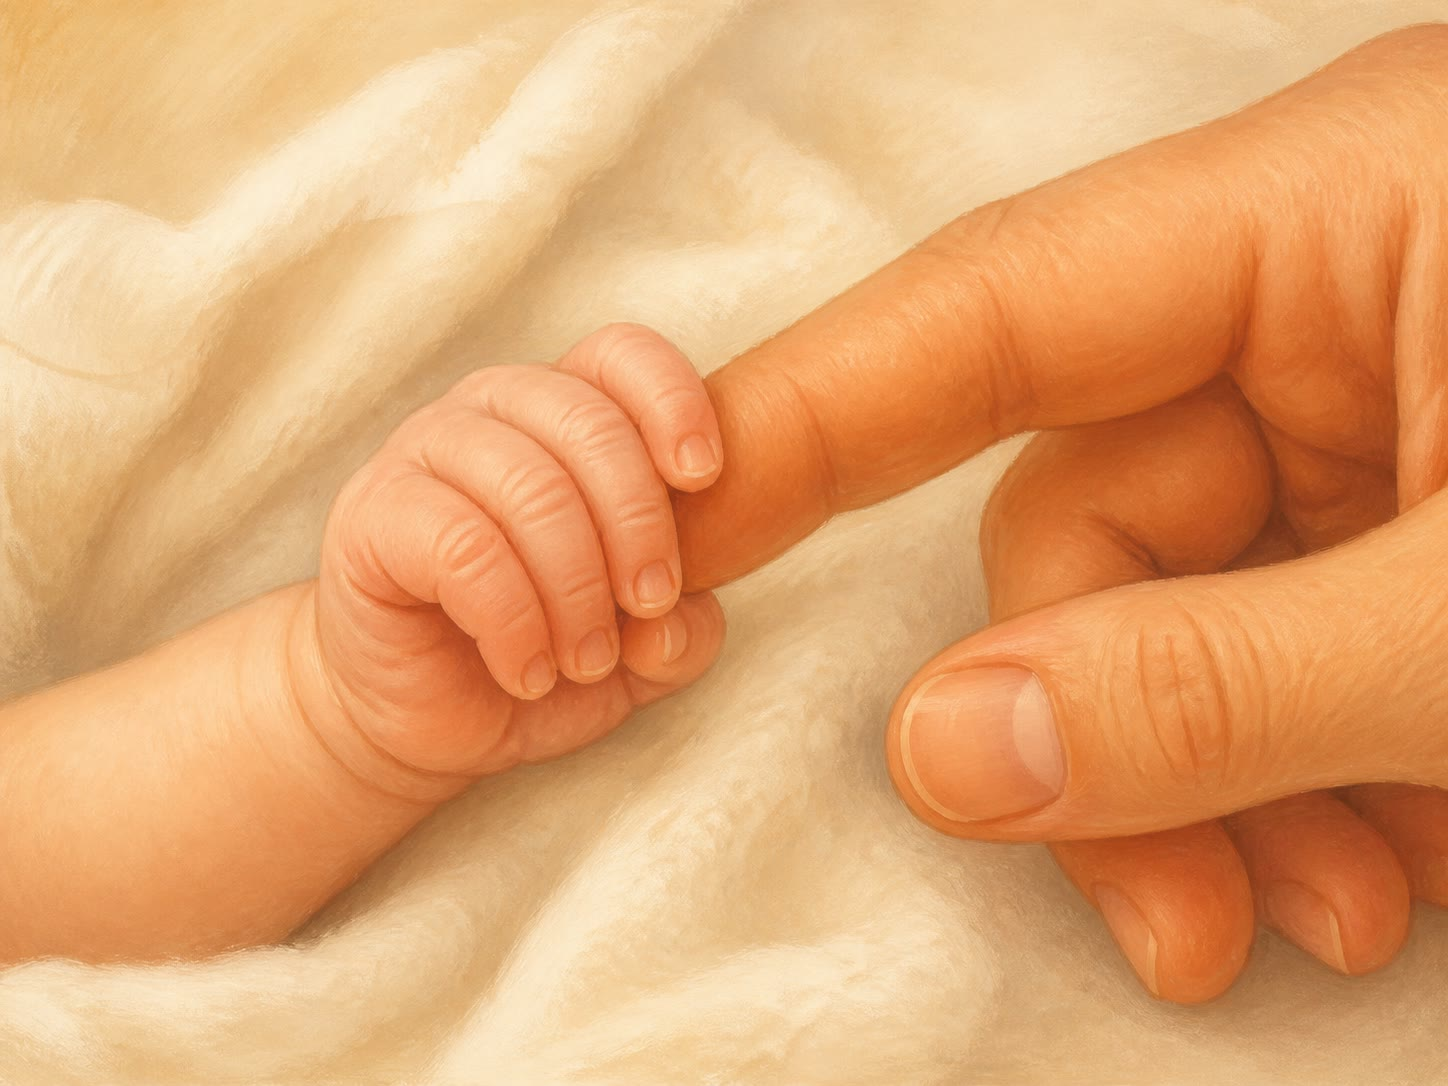
\includegraphics[width=0.52\linewidth]{images/book1/ai/g5-human-babyhand.jpg}

{\small 出生数天后，婴儿的抓握能力已经显现：
人类漫长的童年由此开始。}
\end{omfigure}

\begin{remark}[双胞胎]\label{rem:g5:human-reproduction:twins}
有时，两个婴儿会在\omterm{prop:g5:human-reproduction:plan}{子宫}中同时生长。如果一个
\omterm{def:g5:flower-to-fruit:steps}{受精}卵分裂成两个\omterm{def:g5:human-reproduction:pregnancy}{胚胎}，这对双胞胎就是
\emph{同卵双胞胎}——由同一个起始\omterm{def:g5:first-look-at-cells:cell}{细胞}发育而来，
如同两个相同的复制品。如果两个\omterm{def:g4:animal-reproduction:sexual}{卵细胞}分别与两个
\omterm{def:g4:animal-reproduction:sexual}{精子}结合，这对双胞胎并不比普通兄弟姐妹更相似——
他们只是共享了\omterm{prop:g5:human-reproduction:plan}{子宫}。双胞胎分为两种，
区别在于它们的起源。
\end{remark}

\section{出生前后的照顾}

\begin{proposition}[婴儿与母亲共享营养物质]\label{prop:g5:human-reproduction:care}
所有输送到婴儿体内的物质都要经过母亲的
\omterm{prop:g4:journey-of-food:absorb}{血液}，因此孕妇应吃好
（\cref{ch:g3:balanced-diet}）、多休息，
并接受医生或助产士的随访，避免可能伤害婴儿的东西：烟草烟雾
和酒精同样会通过\omterm{prop:g5:human-reproduction:cord}{脐带}，而且\omterm{def:g5:human-reproduction:pregnancy}{胎儿}
比成人脆弱得多。照顾母亲
\emph{就是}照顾婴儿。
\end{proposition}
\admitted

\begin{example}[极度受到照顾的物种]\label{ex:g5:human-reproduction:longcare}
即使在\omterm{prop:g3:sorting-living-things:groups}{哺乳动物}中，人类也把\cref{prop:g4:animal-reproduction:strategies}
中“少而精心照料”的策略推向了极端：通常一次只生一个婴儿，
无助的时间远比小马驹或小猫长，
并且需要被照料——被喂养、被教导、被
疼爱——持续多\emph{年}。人类的童年是\omterm{def:g1:animals-around-us:animal}{动物}界中最长的之一；
这本书是一门长达十年的课程，
它本身也是这种长期照料的一部分。
\end{example}

\section{练习}

\begin{exercise}[$\star$]\label{exo:g5:human-reproduction:1}
哪个\omterm{def:g5:first-look-at-cells:cell}{细胞}来自母亲，哪个来自父亲，
二者结合的过程叫什么？
\end{exercise}

\begin{exercise}[$\star$]\label{exo:g5:human-reproduction:2}
人类婴儿在哪里生长，大约生长多长时间？
\end{exercise}

\begin{exercise}[$\star$]\label{exo:g5:human-reproduction:3}
生长中的婴儿依次有哪两个名称，
第一个名称大约在何时变成第二个？
\end{exercise}

\begin{exercise}[$\star$]\label{exo:g5:human-reproduction:4}
\omterm{prop:g5:human-reproduction:plan}{子宫}内的婴儿既不进食也不\omterm{def:g4:breathing:movements}{呼吸}。它如何获得\omterm{def:g4:journey-of-food:digestion}{营养物质}和氧气，
废物又去往何处？
\end{exercise}

\begin{exercise}[$\star$]\label{exo:g5:human-reproduction:5}
你的肚脐是什么的痕迹？
\end{exercise}

\begin{exercise}[$\star$]\label{exo:g5:human-reproduction:6}
第一声啼哭时会发生什么？
这对婴儿的身体来说为何是如此大的变化？
\end{exercise}

\begin{exercise}[$\star$]\label{exo:g5:human-reproduction:7}
人类的生殖具有哪些典型的\omterm{prop:g3:sorting-living-things:groups}{哺乳动物}特征？
请列出三个，并参见
\cref{prop:g4:classifying-animals:classes}或
\cref{ch:g4:animal-reproduction}。
\end{exercise}

\begin{exercise}[$\star$]\label{exo:g5:human-reproduction:8}
医生为什么要求孕妇避开烟草烟雾和酒精？
请利用\cref{prop:g5:human-reproduction:care}。
\end{exercise}

\begin{exercise}[$\star\star$]\label{exo:g5:human-reproduction:9}
从形成的方式解释两种双胞胎。哪一种是“如同两个复制品”般相似的，
这一点为何可由
\cref{ex:g5:first-look-at-cells:one}推出？
\end{exercise}

\begin{exercise}[$\star\star$]\label{exo:g5:human-reproduction:10}
将人类放在策略线上，参照
\cref{prop:g4:animal-reproduction:strategies}，与鳕鱼和大象比较：
后代数量、照料时间长短，
以及这种长期照料对人类包含什么内容。
\end{exercise}

\begin{exercise}[$\star\star\star$]\label{exo:g5:human-reproduction:11}
出生时，剪断的\omterm{prop:g5:human-reproduction:cord}{脐带}切断了婴儿的供应通道，
就在肺迎来第一次\omterm{def:g4:breathing:movements}{呼吸}的那一刻。利用
\cref{prop:g5:human-reproduction:cord}和
\cref{prop:g4:breathing:exchange}，解释在这一分钟内，
哪项功能从母体转移到了婴儿自己的肺上，
——以及第一声啼哭为何恰在此时发生。
\end{exercise}
